\normaltrue
\correctionfalse

%\UPSTIidClasse{11} % 11 sup, 12 spé
%\newcommand{\UPSTIidClasse}{12}

\exer{Mouvement RT  $\star$ \label{B2:13:05}}
\setcounter{numques}{0}
\UPSTIcompetence[2]{C2-05}
\UPSTIcompetence[2]{B2-13}
\index{Compétence C2-05}
\index{Compétence B2-13}
\index{Mécanisme à 1 rotation et 1 translation}
\ifcorrection
\else
\textbf{Pas de corrigé pour cet exercice.}
\fi

\ifprof
\else
Soit le mécanisme suivant. On a $\vect{AB}=\lambda(t)\vect{i_1}$.
\begin{center}
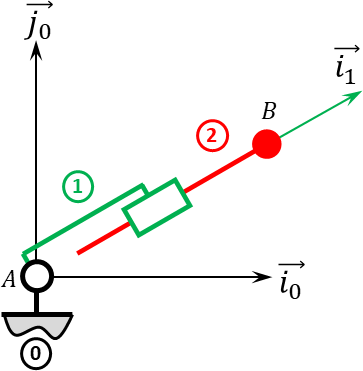
\includegraphics[width=\linewidth]{05_RT_01}
\end{center}
\fi

\question{Donner l'ensemble des positions accessibles par le point $B$.}
\ifprof
En considérant que $\lambda(t)$ peut varier de 0 à $R$ et $\theta(t)$ peut varier de 0 à $2\pi$, toutes les positions du disque de centre $A$ et de rayon $R$ sont accessibles. 
\else
\fi

\question{Donner l'équation horaire (trajectoire en fonction du temps) du point $B$ dans le mouvement de \textbf{2} par rapport à \textbf{0}.}
\ifprof
$\vect{AB}=\lambda(t) \vi{1} =\lambda(t) \cos \theta \vi{0} +\lambda(t) \sin \theta \vj{0}$.  
\else
\fi

On souhaite que le point $B$ réalise un segment entre les points $[-25,25]$ et $[25,25]$. 

\question{Donner les expressions de $\theta(t)$ et $\lambda(t)$ permettant la réalisation de cette trajectoire à la vitesse $v=\SI{0,01}{m.s^{-1}}$.}
\ifprof
On pose $\vect{AB} = x(t)\vi{0}+y(t)\vj{0}$. On a donc 
$\left\{
\begin{array}{l}
x(t) = \lambda(t) \cos \theta(t) \\
y(t) = \lambda(t) \sin \theta(t) \\
\end{array}
\right.$
On note $\ell = 25$. 

Si le segment est parcouru à vitesse constante, on a une durée de parcours de $T = 2\ell / v$. 
Par conséquent la trajectoire souhaitée est donnée par $\forall t \in [0,T]$. 
$\left\{
\begin{array}{l}
x(t) = -\ell+vt \\
y(t) = \ell \\
\end{array}
\right.
$

Par suite,
$\left\{
\begin{array}{l}
-\ell+vt  = \lambda(t) \cos \theta(t) \\
\ell = \lambda(t) \sin \theta(t) \\
\end{array}
\right.$ 
$\Rightarrow 
\left\{
\begin{array}{l}
\left(-\ell+vt\right)^2 + \ell^2   = \lambda(t)^2  \\
\dfrac{\ell}{vt+\ell} =  \tan \theta(t) \\
\end{array}
\right.$ 
$\Rightarrow 
\left\{
\begin{array}{l}
\lambda(t) = \sqrt{\left(-\ell+vt\right)^2 + \ell^2}\\
\theta(t) = \arctan \left( \dfrac{\ell}{vt+\ell} \right)
\end{array}
\right.$ 

\else
\fi


\question{En utilisant Python, tracer $\theta(t)$, $\lambda(t)$ et la trajectoire générée.}
\ifprof
\else
\fi

\ifprof
\else
\begin{flushright}
\footnotesize{Corrigé  voir \ref{B2:13:05}.}
\end{flushright}%
\fi